% !TEX encoding = IsoLatin2
\documentclass[Labor, MSC, german]{twbook}
\usepackage[T1]{fontenc}
% Hier kann je nach Betriebssystem eine der folgenden Optionen notwendig sein, um die Umlaute korrekt wiederzugeben:
% utf8, latin, applemac
\usepackage[utf8]{inputenc}
% Die nachfolgenden 2 Pakete stellen sonst nicht benötigte Features zur Verfügung
\usepackage{blindtext}
\usepackage{listings}
\usepackage{float}

\lstdefinelanguage{PseudoCode}{
    morekeywords={If,wenn,ist,oder,und,Then,Else,EndIf,While,fuer, wiederhole,von, bis,EndWhile,For,EndFor,Function, Funktion,EndFunction},
    sensitive=false,
    morecomment=[l]{//},
    morecomment=[s]{/*}{*/},
    morestring=[b]',
}

\lstset{
    language=PseudoCode,
    basicstyle=\small\ttfamily,
    commentstyle=\itshape\color{gray},
    keywordstyle=\bfseries\color{blue},
    stringstyle=\color{red},
    showstringspaces=false,
    breaklines=true,
    tabsize=4,
    numbers=left,
    numberstyle=\tiny,
    numbersep=5pt,
    frame=single,
    frameround=tttt,
    rulecolor=\color{black},
    captionpos=b,
}

\title{Convex Hull Algorithms \\ (Gift-wrapping, Quick Hull)}
\author{Hannah Kohlhofer, MSc.\and Elias Marcon, MSc. \and Ing. Fabian Steiner, BSc.}
\studentnumber{2310585014 \and 2310585020 \and 2310585027}
\supervisor{FH-Prof. Dipl.-Ing. Alexander Nimmervoll}
%\secondsupervisor{Titel Vorname Name, Titel}
\place{Wien}
\acknowledgements{\blindtext}

\begin{document}
\maketitle

%Algos beschreiben (best/worst case, aufwandsabschätzung anhand der Testbeispiele), Seiten 3-5, Testmessungen

\chapter{Die Algorithmen}
Um die Konvexe Hülle einer Punktemenge zu bestimmen bedarf es verschiedener Algorithmen. Für dieses Projekt implementieren wir zwei verschieden Algorithmen - der Quickhull und der Giftwrapping Algorithmus. Beide Algorithmen haben das Ziel die Konvexe Hülle einer Punktmenge - also das kleinste konvexe Polygon zu bestimmen, wobei hier kein Punkt außerhalb dieser Hülle liegen darf. In anderen Worten: Jeder Punkt der Punktemenge liegt entweder auif der konvexen Hülle oder wird von dieser eingesperrt / umschlossen.



\section{Quickhull}
Der Quick Hull Algorithmus ist dazu da aus einer Punktemenge eine Convexe Hülle zu bilden. Die Grundidee hierbei ist das "Divide and Conquer" Prinzip. Das bedeutet das Gesamtproblem wird zuerst in mehrere Teilprobleme zerlegt und diese werden dann für sich gelöst und abschließen wieder zusammengesetzt um eine Gesamtlösung zu finden.
\subsection{Pseudocode}
\begin{lstlisting}[language=PseudoCode,numbers=left, breaklines=true, caption={Quick Hull Pseudocode \cite{Wikipedia_QuickHull}}]
Funktion QuickHull(S)
{
    // Bestimmt die konvexe Huelle der Menge S
    Convex Hull := {} 
    A := Punkt ganz links
    B := Punkt ganz rechts
    Fuege die Punkte A und B der konvexen Huelle hinzu
    // Die Gerade AB teilt die verbleibenden n - 2 Punkte in die Teilmengen S1 und S2
    S1 := Menge der Punkte in S, die auf der rechten Seite von AB sind
    S2 := Menge der Punkte in S, die auf der linken Seite von AB sind
    FindHull(S1, A, B)
    FindHull(S2, B, A)
    Ausgabe: Convex Hull
}

Funktion FindHull(Sk, P, Q)
{
    // Bestimmt die Punkte auf der konvexen Huelle der Menge Sk, die auf der rechten Seite der Geraden PQ sind
    Wenn Sk keine Punkte enthaelt dann
        Ausgabe: Convex Hull
    C := Der Punkt in Sk, der den groessten Abstand von der Geraden PQ hat
    Fuege den Punkt C in die konvexe Huelle zwischen den Punkten P und Q ein
    // Die drei Punkte P, Q und C teilen die verbliebenen Punkte von Sk in die Teilmengen S0, S1 und S2
    S0 := Die Punkte innerhalb des Dreiecks PCQ
    S1 := Die Punkte auf der rechten Seite der Geraden PC
    S2 := Die Punkte auf der rechten Seite der Geraden CQ
    FindHull(S1, P, C)
    FindHull(S2, C, Q)
    Ausgabe: Convex Hull
}
\end{lstlisting}
Hierbei ist gut zu sehen, wie der Algorithmus das Gesamtproblem aufteilt: beim ersten Aufruf wird die Funktion Quick Hull aufgerufen und diese teilt die Menge der Punkte in der Hälfte auf und ruft damit jeweils einmal die Funktion FindHull auf, welche die Punkte wieder aufteilt und sich mit den zwei Hälften selbst erneut aufruft.
\subsection{Beschreibung des Alogrithmus}
Der Algorithmus beginnt damit, dass er den linkesten und den rechtesten Punkt auswählt und sie zur konvexen Hülle hinzufügt. Dadruch entsteht eine Linie (im Pseudocode bezeichnet als $AB$). Nun wird für die Punktemenge auf jeder Seite der Hülle weiter betrachtet. Man sucht hier nun jeweils nach dem am weitesten entfernten Punkt $C$ zur Geraden. Die Auswahl des am weitesten Entfernten Punktes führt hier zu den Besten Ergebnissen, wie in "The Quickhull Algorithm for Convex Hulls"\cite{10.1145/235815.235821} beschrieben wird. Man verbindet nun die Gerade $AB$ mit dem Punkt $C$ und erhält dadurch ein Dreieck ($S0$) in dem sich (wahrscheinlich) Punkte befinden, die nicht mehr weiter betrachtet werden müssen (da sie schon innerhalb der Hülle liegen). Wenn sich außerhalb des Dreiecks linkerseits zu $AC$ und rechterseits zu $BC$ Punkte befinden, wird für diese der Schritt "FindHull" wiederholt, bis sich alle Punkte in der Hülle befinden.
\subsection{Aufwandsabschätzungen und Testfälle}
\subsubsection{Theorie}
Laut Barber, Dobkin und Huhdanpaa \cite{10.1145/235815.235821} liegt die oberste Schranke bei $\mathcal{O}(n * log( n))$, wenn die Pivotpunkte gut gewählt werden (zum Beispiel der am weitesten entfernte Punkt). Werden sie zufällig gewählt, so liegt die oberste Schranke im 2D bei $\mathcal{O}(n^2)$.

\subsubsection{Messwerte}
\begin{figure}[H]
    \centering
    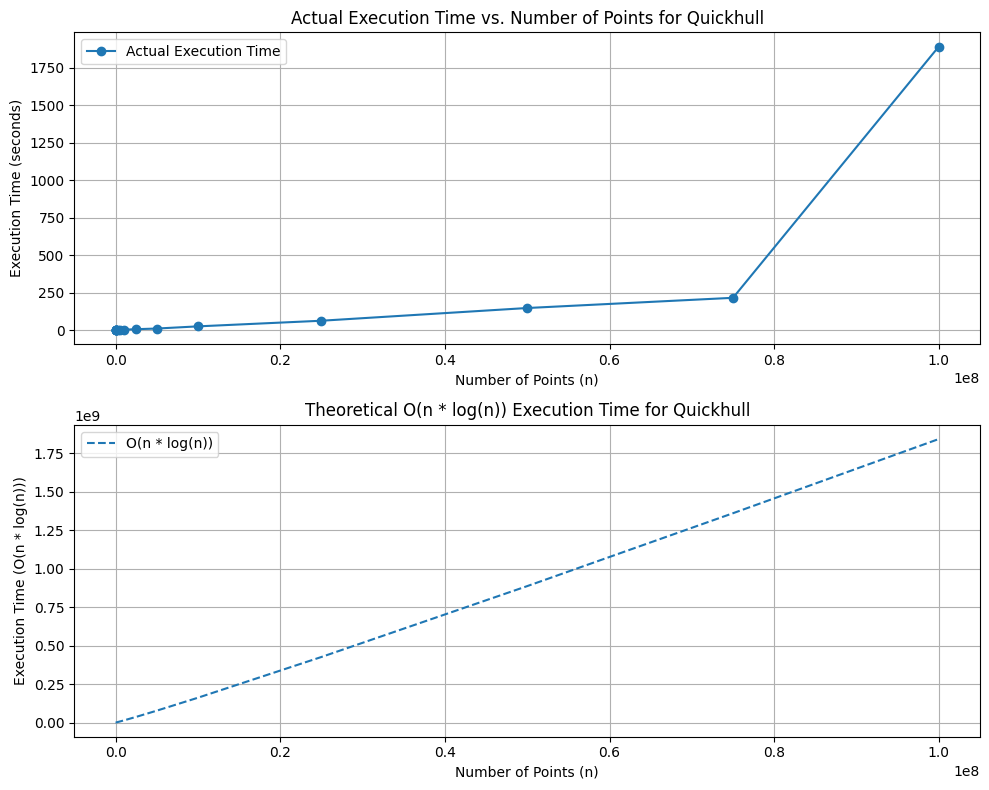
\includegraphics[width=0.6\textwidth]{./PICs/QuickHull.png}
    \caption{QuickHUll: Vergleich von Messwerten (oberer Graph) mit $\mathcal{O}(n* log(n))$}
    \label{fig:quickHull}
\end{figure}
Der Algorithmus verhält sich nur bei gewissen (balancierten) Eingaben $\mathcal{O}(n* log(n))$, bei unbalancierten Eingaben geht das Verhalten gegen $\mathcal{O}(n^2)$. Allerdings ist auch festzuhalten, dass durch die Implementierung in Python nie eine optimale Laufzeitmessung erreicht werden kann, sich der Verlauf der Laufzeit jedoch schon beobachten lässt. Erschwerend kommt hinzu, dass bei hohen Datenmengen die Begrenzung der Hardware (RAM) schlagend wird - damit könnte man auch den plötzlichen Anstieg erklären.



\section{Giftwrapping}
Der Giftwrapping Algorithmus, dient, wie zuvor beschrieben, ebenfalls zur Berechnung der Konvexen Hülle (CH) einer Punktemenge (Q). Im Zwei-Dimensionalen Fall wird der Giftwrapping Algorithmus auch als Jarvis-March bezeichnet, benannt nach seinem "Entdecker"  R. A. Jarvis im Jahr 1973 (siehe \cite{JARVIS197318}).

\subsection{Pseudocode}
Im Folgenden Code geltend die Bezeichnungen P für den jeweiligen Startpunkt und S für die gesamte Punktemenge.

\begin{lstlisting}[language=PseudoCode,numbers=left, breaklines=true, caption={Giftwrapping Pseudocode \cite{Wikipedia_GiftWrapping}}]
    startpunkt = Punkt mit kleinster Ordinate
    i = 0
    wiederhole
        P[i] = startpunkt
        endpunkt = S[0]
        wenn startpunkt == endpunkt
          endpunkt = S[1]
        fuer j von 1 bis |S|
          ist (endpunkt == startpunkt) oder (S[j] links von der Geraden zwischen startpunkt und endpunkt)
            endpunkt = S[j]
        startpunkt = endpunkt
        i++
    bis endpunkt == P[0]
\end{lstlisting}

    
\subsection{Beschreibung des Algorithmus}
Der Giftwrapping Algorithmus startet beim untersten Punkt der Punktemenge $p$ (kleinster $y$-Wert). Sollten mehrere Punkte den gleichen $y$-Wert aufweisen, so wird jener Punkt gewählt, der zusätzlich den kleinsten $x$-Wert aufweist. Dann werden iterativ alle anderen Punkte mittels des Winkels von $p$ sortiert. Der Punkt mit dem kleinsten Winkel ($a$) liegt demzufolge auf der konvexen Hülle und kann mit dem Ausgangspunkt verbunden werde. Infolgedessen steht Punkt $a$ als neuer Ausgangspunkt zur Verfügung und es werden erneut alle Winkel von diesem Punkt aus berechnet. So wiederholt sich der Algorithmus, bis am Ende die Konvexe Hülle geformt werden kann.\\

Die Bezeichnung "Winkel berechnen" kann hierbei etwas irreführend sein. Um den Algorithmus zu vereinfachen werden nicht tatsächliche Winkelwerte berechnet, sondern es werden einfache gerade Linien vom Ausgangspunkt P zu allen anderen Punkten gezogen. Es wird somit für jeden Punkt bzw. jede gerade überprüft, ob sich links von dieser Gerade noch eine weitere befindet. Sollte dies der Fall sein, wird jeweils die "linkeste Gerade" für die Konvexe Hülle verwendet, solange keine neue gefunden wird, die noch weiter links ist. Der Algorithmus arbeitet sich also entgegen dem Uhrzeigersinn voran, bis die gesamt Konvexe Hülle gebildet ist.

\subsection{Aufwandsabschätzungen und Testfälle}
\subsubsection{Theorie}
Laut Jarvis (\cite{JARVIS197318}) hat der Giftwrapping Algorithmus einen Aufwand von $\mathcal{O}(n(h+1))$, für $n$ Punkt in der Punktmenge und $n\leq h$ auf der Hülle liegende Punkte. Andere Quellen berichten von einer Laufzeit von $\mathcal{O}(nh)$. In den meisten Fällen, wird jedoch nicht einmal dieser Aufwand benötigt werde, da der Algorithmus vereinfacht werden kann, sowohl durch den zuvor beschriebenen Austausch der Winkelberechnungen mit simplen Checks auf welcher Seite ein Punkt liegt, als auch durch den gezielten Ausschluss von Punkten für alle weiteren Berechnungen. Punkte werden somit ausgeschlossen, wenn sie entweder bereits als auf der konvexen Hülle liegend bestimmt wurden, oder sie in dem Bereich liegen, der vom ersten zum letzten Punkt auf der Hülle eingegrenzt wird. Diese Vereinfachung ist im Pseudocode nicht zu sehen, kann jedoch ganz einfach implementiert werden.\\

Die Laufzeit des Giftwrapping Algorithmus hängt von der Größe des Outputs ab, was ihn zu einem sogenannten "output sensitive" Algorithmus macht. Wie im vorherigen Absatz erwähnt, hängt der Algorithmus linear von der Anzahl der Punkte auf der Hülle ab. Demnach kann die Laufzeit nur dann, wie bei anderen Algorithmen, gleich schnell oder schneller als $\mathcal{O}(nlog(n))$ sein, wenn die Anzahl der auf der Hülle liegenden Punkte $h$ kleiner ist als $nlog(n)$. Der Idealfall, für die kürzest Mögliche Laufzeit würde eintreten, wenn immer direkt der linkeste Punkt gefunden wird. Der "Best Case" hat somit eine Laufzeit von $\mathcal{O}(n)$. Der "Worst Case" hingegen tritt ein, wenn alle Punkte auf einem Kreis liegen. In diesem Fall ist 
$h=n$ und somit beträgt die Laufzeit $\mathcal{O}(n^2)$, da jeder Punkt mit jedem Punkt verglichen werden muss.

\subsubsection{Messwerte}
\begin{figure}[H]
    \centering
    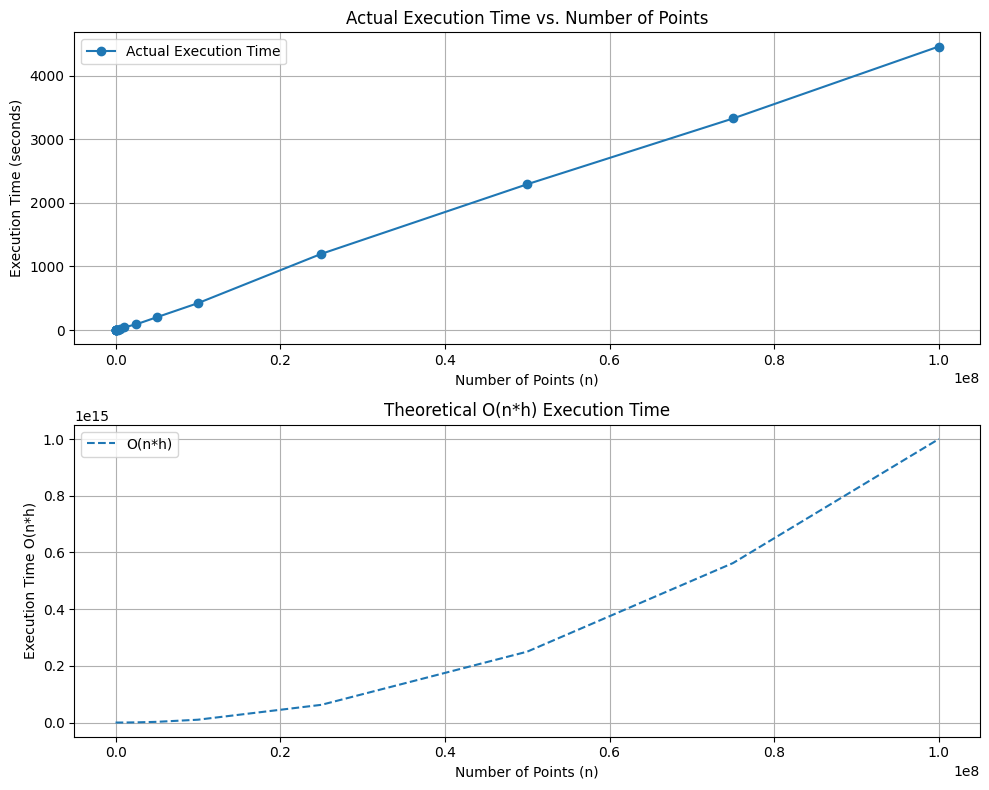
\includegraphics[width=0.6\textwidth]{./PICs/Giftwrapping.png}
    \caption{Giftwrapping: Vergleich von Messwerten bei verschiedenen Testfällen des Giftwrapping Algorithmus. Der obere Graph zeigt die tatsächliche Laufzeit des Algorithmus mit $\sim\mathcal{O}(n)$. Im unteren Graph ist die theoretische Laufzeit von  $\mathcal{O}(n*h)$ abgebildet.}
    \label{fig:gitwrapping}
\end{figure}

Auch wenn man in Abbildung \ref{fig:gitwrapping} zu erkennen vermag, dass der Algorithmus immer eine ideale Laufzeit von $\mathcal{O}(n)$ hat, gibt es wie fast immer Ausnahmen. Betrachtet man den Bereich mit sehr wenigen Punkten, so sieht man, dass hier auch teilweise eine stärkere Steigung aufgewiesen wird als linear. Dies hängt natürlich auch mit der bereits zuvor erwähnten schwächeren Leistung von Python im Vergleich zu C++ zusammen, kann aber natürlich auch einen Ursprung im Algorithmus bzw. seiner Implementierung finden.\\

Zusammenfassend kann hier festgehalten werden, dass sich unser Algorithmus nahe der idealen Laufzeit von $\mathcal{O}(n)$ bewegt und somit besser ist als theoretisch (im Mittel) erwartet wird. Warum genau das so ist, ist jedoch schwer zu sagen.



\clearpage
\bibliography{Literatur}
\bibliographystyle{plain}

\clearpage

% Das Abbildungsverzeichnis
\listoffigures
\clearpage


\end{document}